%!TEX root = ../Base.tex

%*****************************************
\chapter{Hidden Markov Model}\label{ch:chap2}
%*****************************************

Cuando se tienen secuencias de datos o datos secuenciales, se pueden agrupar 
en dos tipos, dependiendo de sus características: distribuciones estacionarias 
y distribuciones no estacionarias.

En el caso de secuencias de datos estacionarias, los datos \textit{evolucionan}
a través del tiempo, pero la distribución a partir de la cuál fueron generados 
permanece igual; mientras que para el caso de datos no estacionarios, su distribución 
generativa va variando también según pasa el tiempo.

Para el problema de \sd así como la detección de fraude en tarjetas de crédito, consideraremos 
que los datos son estacionarios; por lo que entonces su distribución generativa no cambia, 
y es la que se tratará de modelar y ajustar para resolver estos problemas.

Este tipo de datos, permiten modelar una gran cantidad de situaciones, en las que se
tienen observaciones de acuerdo al tiempo, y se puede predecir el siguiente valor en
la serie dadas la observaciones que se tienen hasta el momento.

De forma general, se suelen considerar únicamente las observaciones más recientes, 
pues son las que pudiéramos pensar son más informativas para la predicción; 
además de que al asumir que las predicciones de nuevos datos sólo dependen de las últimas 
observaciones permite simplificar mucho el modelo de la distribución generativa.

Para trabajar con este tipo de datos, se puede usar entonces un modelo de Márkov, en el 
que se asume la independecia de las predicciones futuras con todas las observaciones 
excepto las últimas.

\section{Modelo de Markov}

El modelo generativo más sencillo que se podría pensar, es considerar que todas las 
observaciones son independientes, es decir, que son i.i.d, cuyo modelo gráfico se muestra
en la \autoref{fig:mod_iid}.

\begin{figure}[bt]
        \myfloatalign
        {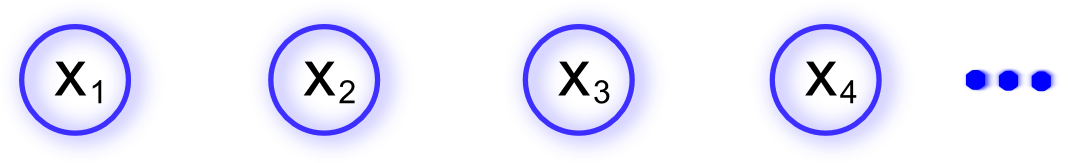
\includegraphics[width=0.6\linewidth]{gfx/3-mod-iid}}        
        \caption{Observaciones independientes e idénticamente distribuidas.}
        \label{fig:mod_iid}
\end{figure}

Al asumir que los datos no están relacionados, sin embargo, se llega a perder gran cantidad 
de información relativa al orden en que se fueron dando estas observaciones.

Es decir, si se tiene un conjunto $N$ de observaciones $\mb{X} = \lbrace x_1, ..., x_n \rbrace$, 
y se asume que son i.i.d, la distribución conjunta de la secuencia de datos se
puede escribir como sigue:
\begin{equation}
\label{eqn:3-1}
p(x_1, ..., x_N) ~=~ \prod_{n=1}^N p(x_n)
\end{equation}

En cambio, para expresar la dependencia entre un grupo de observaciones secuenciales, 
se puede utilizar entonces un modelo probabilístico llamado \textit{modelo de Markov}, 
en el que usando la regla del producto \graffito{Dar ejemplo de regla} se expresa 
la distribución conjunta de las observaciones de la siguiente manera:
\begin{equation}
\label{eqn:3-2}
p(x_1, ..., x_N) ~=~ \prod_{n=1}^N p(x_n ~|~ x_1, ..., x_{n-1}).
\end{equation}

Ahora, si se asume que cada $x_n$ es independiente de las observaciones anteriores 
excepto de la más reciente $x_{n-1}$, se tiene que la distribución conjunta se 
puede escribir de forma más sencilla utilizando el teorema de separación D, puesto que 
\begin{equation}
\label{eqn:3-3}
p(x_n ~|~ x_1, ..., x_{n-1}) ~=~ p(x_n ~|~ x_{n-1})
\end{equation}
entonces el modelo probabilístico se le conoce como cadena de Márkov de primer orden 
y sería el siguiente
\begin{equation}
\label{eqn:3-4}
p(x_1, ..., x_N) ~=~ p(x_1) \prod_{n=2}^N p(x_n ~|~ x_{n-1}).
\end{equation}
y su modelo gráfico corresponde a la \autoref{fig:mod_mm1}
\begin{figure}[bt]
        \myfloatalign
        {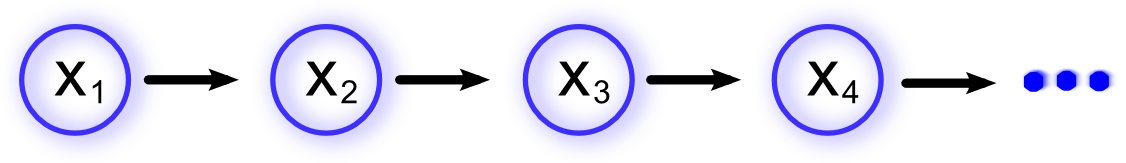
\includegraphics[width=0.6\linewidth]{gfx/3-mod-mm1}}
        \caption{Modelo de Márkov de primer orden.}
        \label{fig:mod_mm1}
\end{figure}

Para el caso en el que los datos provienen de un modelo estacionario, se dice que 
la cadena de Márkov es \textit{homogénea}, puesto que las probabilidades condicionales 
$p(x_n ~|~ x_{n-1})$ son fijas.

Aunque en este caso, el modelo es mucho más general que el asumir que todas las 
observaciones son independientes; aún el modelo es ciertamente restrictivo. 

De la misma manera en que se consideró para cuando $x_n$ depende únicamente de 
la observación anterior, se puede extender este proceso para por ejemplo, que 
$x_n$ dependa sólo de las dos observaciones previas. A este modelo  se le conoce 
como cadena de Márkov de segundo orden; y usando de la misma manera el teorema 
de separación D, la distribución conjunta de las observaciones se puede escribir como 
\begin{equation}
\label{eqn:3-5}
p(x_1, ..., x_N) ~=~ p(x_1) \cdot p(x_2 ~|~ x_1) \prod_{n=3}^N p(x_n ~|~ x_{n-1}, x_{n-2})
\end{equation}
puesto que se tiene que $x_n \perp x_1, ..., x_{n-3} ~|~ x_{n-1}, x_{n-2}$.
En este caso su modelo gráfico correspondiente es la \autoref{fig:mod_mm2}, en el que 
se puede observar la dependencia de una $x_n$ en específico únicamente con sus 
dos observaciones anteriores.

\begin{figure}[bt]
        \myfloatalign
        {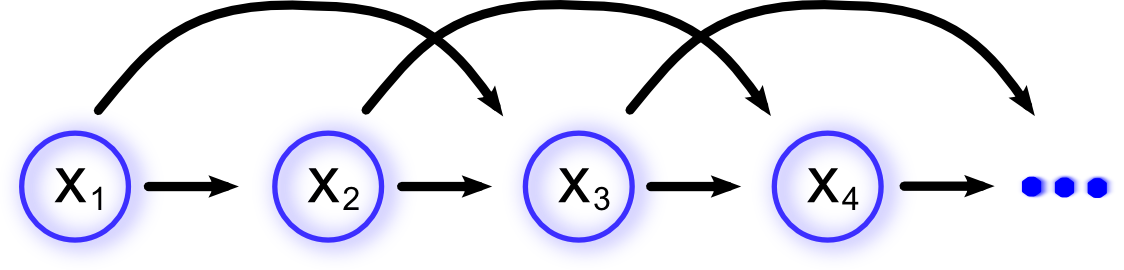
\includegraphics[width=0.6\linewidth]{gfx/3-mod-mm2}}
        \caption{Modelo de Márkov de segundo orden.}
        \label{fig:mod_mm2}
\end{figure}

De la misma forma se puede generalizar para cualquier $M$ con modelos de Márkov 
de $M$-ésimo orden, aunque el considerar demasiados estados previos puede complicar
demasiado el modelo; pues el número de parámetros implicados aumenta de forma 
exponencial al orden del modelo de Márkov.

Para evitar que el modelo se vuelva demasiado complejo, así como para no hacer 
alguna suposición a priori sobre de qué orden es del modelo generativo, se puede 
introducir una variable oculta, que permita cambiar el planteamiento del modelo. 
Se considera entonces una variable latente $z_n$ correspondiente a cada observación 
$x_n$, y entonces el conjunto de variables latentes forman una cadena de Márkov, 
como se muestra en la \autoref{fig:mod_hmm1}

Se asumirá entonces 
\begin{equation}
\label{eqn:3-6}
z_{n+1} \perp z_{n-1} ~|~ z_{n}
\end{equation}

Y entonces, usando la regla de la cadena, la distribución conjunta para este modelo
es la siguiente: 

\begin{equation}
\label{eqn:3-7}
p(x_1, ..., x_N, z_1, ..., z_N) ~=~ p(z_1) \left [ \prod_{n=2}^N p(z_n ~|~ z_{n-1}) \right ] 
\prod_{n=1}^N p(x_n ~|~ z_{n}).
\end{equation}

\begin{figure}[hbt]
        \myfloatalign
        {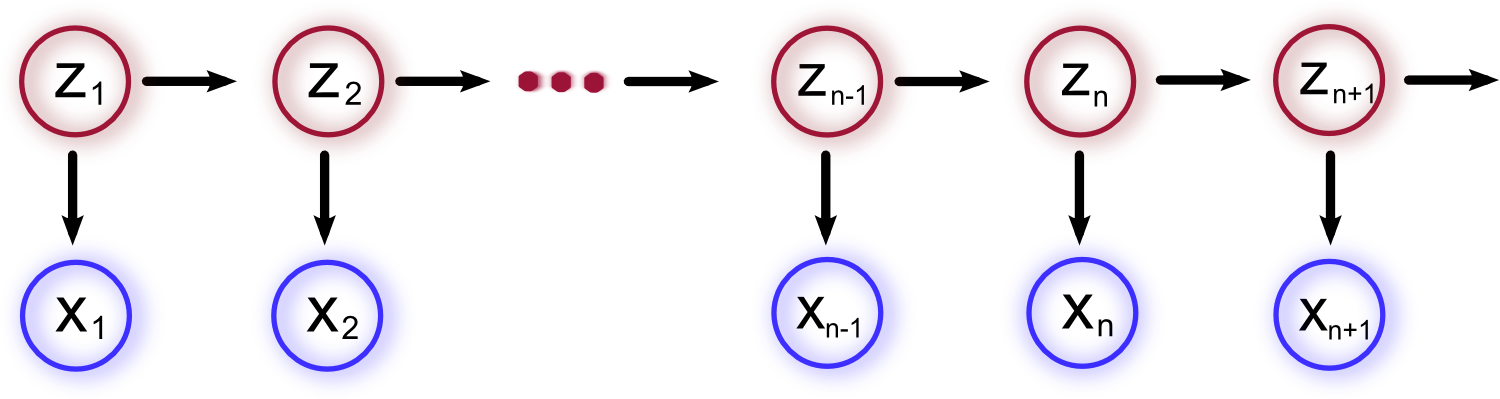
\includegraphics[width=0.8\linewidth]{gfx/3-mod-hmm}}
        \caption{Modelo oculto de Márkov.}
        \label{fig:mod_hmm1}
\end{figure}

Para éste último modelo gráfico, si las variables latentes son discretas, entonces se le 
conoce como Modelo oculto de Márkov o HMM (\textit{Hidden Markov Model}), y es justo el 
modelo que se utilizará para la tarea de \sd.

\section{HMM}

Un modelo oculto de Márkov, sigue siendo entonces un modelo para datos secuenciales, en 
los que además se introduce el concepto de una variable oculta de la cual dependen las 
observaciones que se tienen; y de forma más especifica, esta variable oculta es discreta. 

Usando un HMM entonces podemos modelar un proceso bivariado discreto en el tiempo, con ciertas 
propiedades interesantes que permiten 

Para cada instante de tiempo en el HMM, se le puede considerar como una mezcla de distribuciones
en la que la densidad tiene un distribución dada por $p(x|z)$, es decir, la mezcla de los 
componentes está dada por las observaciones previas.

Se puede considerar entonces, que cada variable latente $z_n$ tendrá una distribución 
multinomial discreta, que indicará cuál componente de la mezcla de distribuciones es la 
que ha generado la observación $x_n$. Para ésto, se usará la notación \unk, que corresponde 
a un conjunto de variables indicador $z_{nk} \in \lbrace 0, 1 \rbrace$, donde $k = 1, ..., K$ 
señalando cuál de las $K$ distribuciones generó a la variable $x_n$, \ie, si el componente 
generador de $x_n$ fue la $k$-ésima mezcla, entonces $z_{nk} = 1$ y $z_{nj} = 0$ para todo 
$j \neq k$.

Ahora, se tiene que cada variable $z_n$ depende únicamente de $z_{n-1}$, y puesto que 
las variables latente son vectores binarios de $K$ dimensiones, entonces se tendría que 
la probabilidad condicional de $z_n ~|~ z_{n-1}$ se puede representar mediante una tabla 
o matriz, que se denotará como $\mb{A}$, y será referida como \textit{matriz de 
probabilidades de transición}. 

Los componentes de la matriz de transición se definen tal que $A_{jk} \equiv p(z_{nk} = 1 ~|~  z_{n-1, j} = 1)$, 
y puesto que son probabilidades, se cumple que $0 \leq A_{jk} \leq 1$ además de que 
$\sum_k A_{jk} = 1$. Considerando estas restricciones, entonces la matriz $\mb{A}$ 
tiene $K (K-1)$ parámetros independientes.

Se puede escribir entonces la probabilidad condicional de una variable latente $z_n$ 
dada la anterior variable latente $z_{n-1}$ de la siguiente forma: 
\begin{equation}
\label{eqn:3-8}
p(z_n ~|~ z_{n-1}, \mb{A}) = \prod_{k=1}^K \prod_{j=1}^K A_{jk}^{z_{n-1, j} \cdot z_{nk}}
\end{equation}

Además, se tiene que considerar la variable latente inicial $z_1$, puesto que ésta no 
tiene una variable latente anterior, la \autoref{eqn:3-7} no aplica; por lo que entonces 
la probabilidad marginal de $z_1$ está representada por un vector de probabilidades $\pi$ 
tal que $\pi_k \equiv p(z_{1k})$, por lo que se puede reescribir como sigue: 
\begin{equation}
p(z_1 ~|~ \pi) = \prod_{k=1}^K \pi_k^{z_{1k}}
\end{equation}
y además se cumple que $\sum_k \pi_k = 1$ por definición.

La matriz de transición también se puede llegar a representar como un grafo dirigido, si 
se consideran las entradas de la matriz $\mb{A}$ como los pesos de las aristas, y los 
nodos son cada uno de los posibles $K$ estados. Por ejemplo, para el caso de una variable 
latente de $K = 3$ estados, se tendría el grafo de la \autoref{fig:mod_hmm2}.

\begin{figure}[hbt]
        \myfloatalign
        {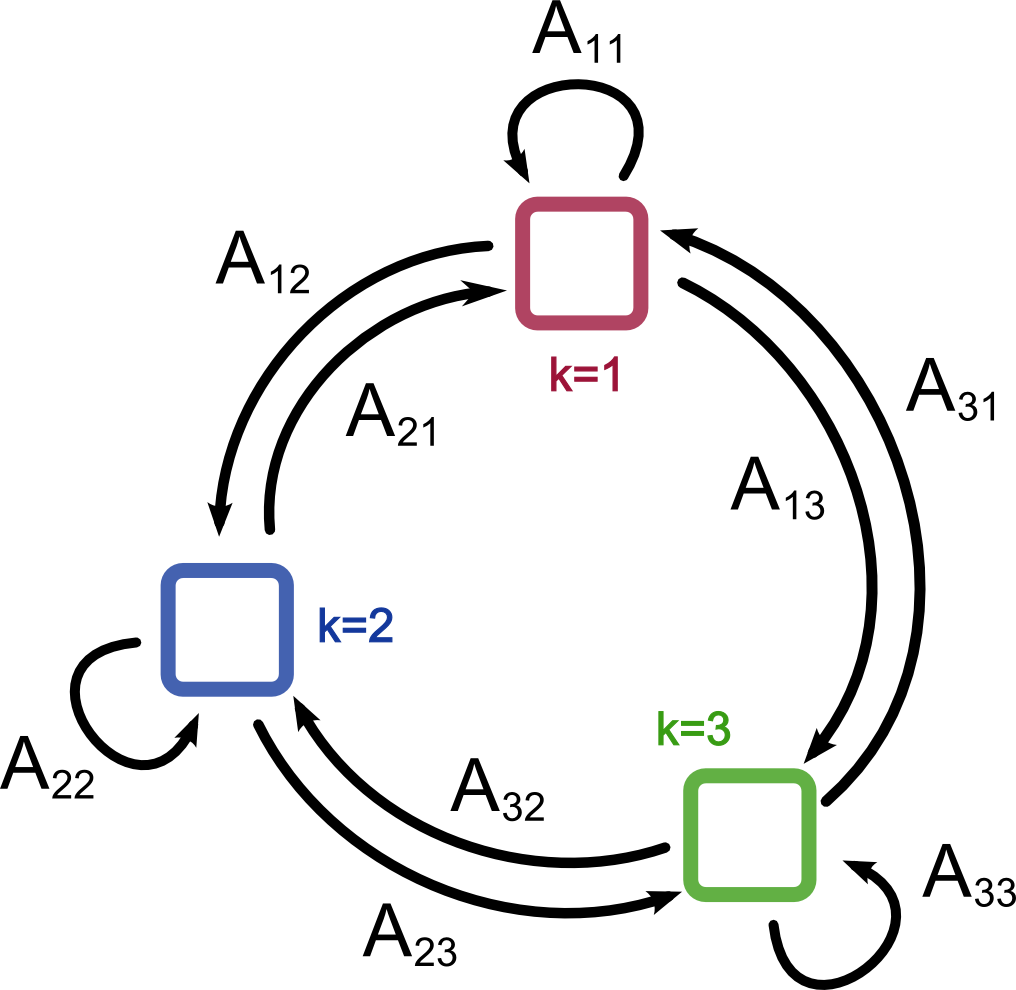
\includegraphics[width=0.4\linewidth]{gfx/3-mod-hmm2}}
        \caption{Modelo oculto de Márkov.}
        \label{fig:mod_hmm2}
\end{figure}

De la misma manera, el grafo correspondiente a la matriz de transición, se puede representar 
como una rejilla a través del tiempo, en la que se mantienen los vértices y aristas del grafo, 
pero además se introduce la noción del tiempo. Como se observa en la \autoref{fig:mod_hmm3} 

\begin{figure}[hbt]
        \myfloatalign
        {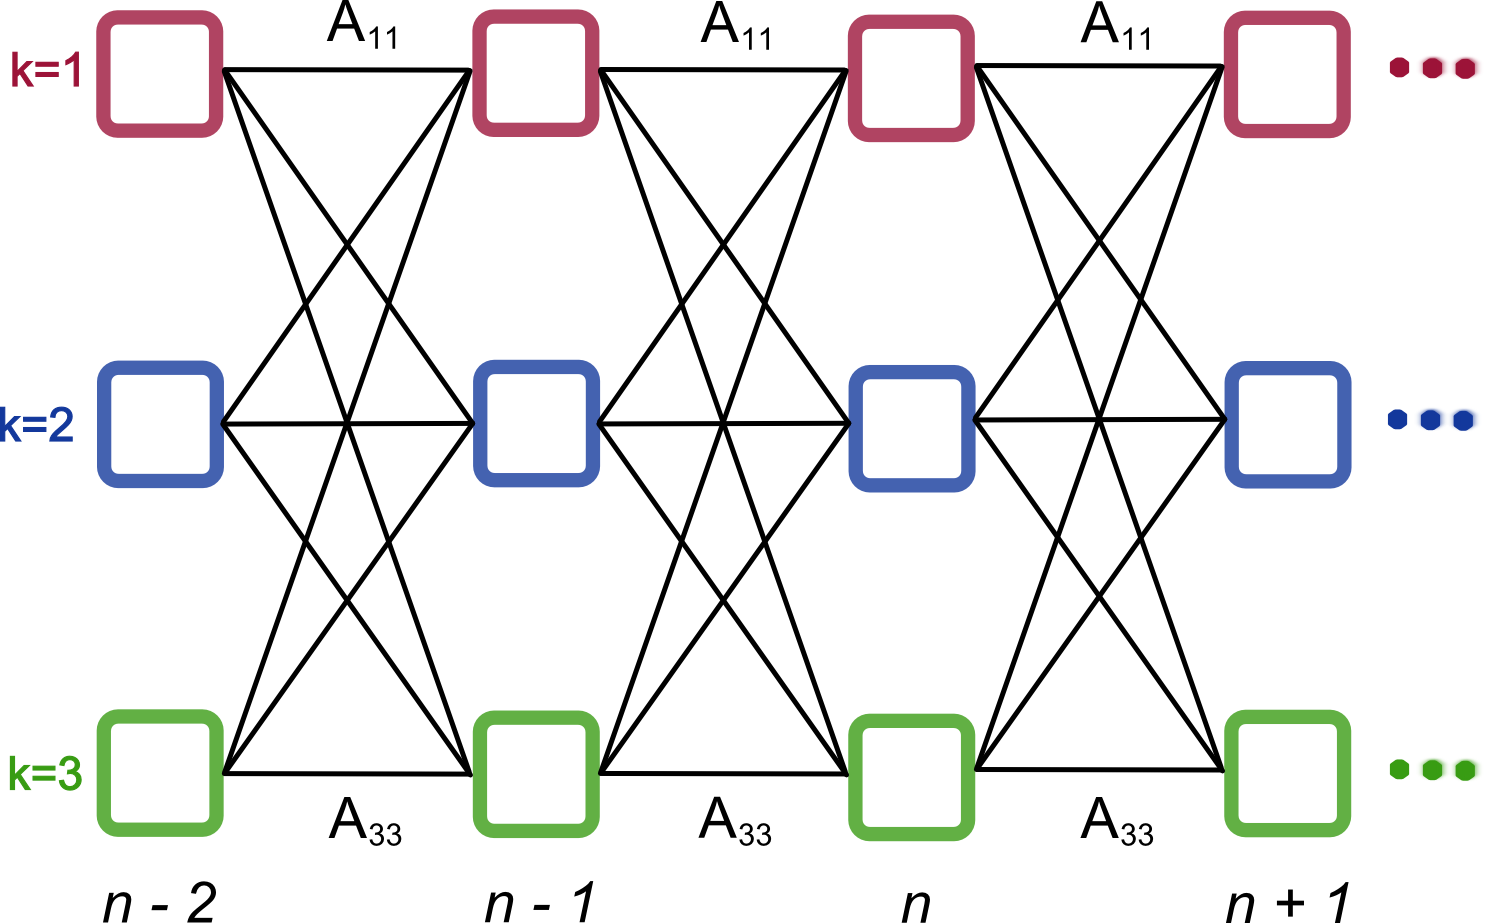
\includegraphics[width=0.63\linewidth]{gfx/3-mod-hmm3}}
        \caption{Modelo oculto de Márkov.}
        \label{fig:mod_hmm3}
\end{figure}

Por último, para completar el modelo se tiene que considerar además la distribución condicional 
de las variables observadas, es decir $p(x_n ~|~ z_n, \phi)$ donde $\phi$ es un conjunto de 
parámetros específicos a la distribución de $x$. Se les conoce como probabilidades de emisión, 
y puede ser tanto una distribución discreta como una continua. Para el caso en que la probabilidad
de emisión esté dada por una distribución discreta, entonces se tendrá una tabla de probabilidades.

Para calcular entonces esta probabilidad de emisión, se tiene tanto $z_n$ como unos parámetros $\phi$ 
dados, por lo que entonces se tienen un vector de $K$ valores para cada uno de los posibles estados del 
vector indicador $z_n$.

Se puede escribir entonces la probabilidad de emisión como sigue:
\begin{equation}
p(x_n ~|~ z_n, \phi) = \prod_{k=1}^K p(x_n ~|~ \phi_k) ^ {z_{nk}}
\end{equation}
y entonces la probabilidad conjunta quedaría definida de la siguiente manera:
\begin{equation}
p(\mb{X}, \mb{Z} ~|~ \theta) 
= p(z_1 ~|~ \pi) \left[ \prod_{n=2}^N p(z_n ~|~ z_{n-1}, \mb{A}) \right]
\prod_{n=1}^N p(x_n ~|~ z_n, \phi)
\label{eqn:3-11}
\end{equation}
donde $\mb{X} = \lbrace x_1, ..., x_N \rbrace$,~ $\mb{Z} = \lbrace z_1, ..., z_N \rbrace$~ y ~
$\theta = \lbrace \pi, \mb{A}, \phi \rbrace$ es el conjunto de parámetros requeridos por el modelo.

La intuición del modelo oculto de Márkov se puede entender más fácilmente si se revisa desde el punto de
vista generativo. Primero, se muestrea la variable latente inicial $z_1$, de acuerdo a las probabilidades 
$\pi_k$, así como su correspondiente $x_1$. Luego, se debe escoger un $z_2$. Para esto, si se supone que 
$z_1$ es igual a algún estado $j$, entonces usando la matriz de transición se muestrea $z_2$ con probabilidades 
$A_{jk}$ para $k = 1, ... , K$, y de igual manera, su correspondiente variable observada $x_2$. Éste mismo
proceso es el que se sigue para cada iteración en el tiempo, hasta que se forma completamente el modelo 
oculto de Márkov y se le conoce como \textit{muestreo ancestral} y se suele usar para modelos con grafos dirigidos.

Si la matriz de transición es predominantemente diagonal, entonces en la secuencia de datos puede que un mismo 
estado $i$ sea el que genere muchos puntos $x_n$, pues con poca probabilidad cambiará de un estado $i$ a $j$. 
Este fenómeno es justo el que se espera para el caso de \sd, pues usualmente una persona $p_i$ hablará
durante mucho tiempo, y luego cuando otra persona $p_j$ toma la palabra, sucederá lo mismo.